
\documentclass[letterpaper,hide notes,xcolor={table,svgnames},pdftex,10pt]{beamer}
\def\showexamples{t}

\usecolortheme{crane}
\setbeamertemplate{navigation symbols}{}

\usetheme{MyPittsburgh}
\usepackage{hyperref}
\usepackage{graphicx,xspace}
\usepackage[normalem]{ulem}
\usepackage{multicol}
\usepackage{amsmath,amssymb,amsthm,graphicx,xspace}
\newcommand\SF[1]{$\bigstar$\footnote{SF: #1}}

\usepackage[sfdefault,lf]{carlito}
\usepackage[T1]{fontenc}
\usepackage[scaled]{beramono}
\usepackage{tikzpagenodes}
\newcommand{\Rplus}{\protect\hspace{-.1em}\protect\raisebox{.35ex}{\small{\small\textbf{+}}}}
\newcommand{\Cpp}{\mbox{C\Rplus\Rplus}\xspace}

\newcounter{tmpnumSlide}
\newcounter{tmpnumNote}

\newcommand\mnote[1]{%
	\addtocounter{tmpnumSlide}{1}
	\ifdefined\showcues {~\tiny\fbox{\arabic{tmpnumSlide}}}\fi
	\note{\setlength{\parskip}{1ex}\addtocounter{tmpnumNote}{1}\textbf{\Large \arabic{tmpnumNote}:} {#1\par}}}

\newcommand\mmnote[1]{\note{\setlength{\parskip}{1ex}#1\par}}


\newcommand\mquestion[2]{{~\color{red}\fbox{?}}\note{\setlength{\parskip}{1ex}\par{\Large \textbf{?}} #1} \note{\setlength{\parskip}{1ex}\par{\Large \textbf{A}} #2\par}\ifdefined \presentationonly \pause \fi}

\newcommand\blackboard[1]{%
	\ifdefined   \showblackboard
		{#1}
	\else {\begin{center} \fbox{\colorbox{blue!30}{%
						\begin{minipage}{.95\linewidth}%
							\hspace{\stretch{1}} Some space intentionally left blank; done at the blackboard.%
						\end{minipage}}}\end{center}}%
	\fi%
}

\usepackage{listings}
\lstset{%
	keywordstyle=\bfseries,
	aboveskip=15pt,
	belowskip=15pt,
	captionpos=b,
	identifierstyle=\ttfamily,
	frame=lines,
	numbers=left, basicstyle=\scriptsize, numberstyle=\tiny, stepnumber=0, numbersep=2pt}

\usepackage{siunitx}
\newcommand\sius[1]{\num[group-separator = {,}]{#1}\si{\micro\second}}
\newcommand\sims[1]{\num[group-separator = {,}]{#1}\si{\milli\second}}
\newcommand\sins[1]{\num[group-separator = {,}]{#1}\si{\nano\second}}
\sisetup{group-separator = {,}, group-digits = true}

%% -------------------- tikz --------------------
\usepackage{tikz}
\usetikzlibrary{positioning}
\usetikzlibrary{arrows,backgrounds,automata,decorations.shapes,decorations.pathmorphing,decorations.markings,decorations.text}

\tikzstyle{place}=[circle,draw=blue!50,fill=blue!20,thick, inner sep=0pt,minimum size=6mm]
\tikzstyle{transition}=[rectangle,draw=black!50,fill=black!20,thick, inner sep=0pt,minimum size=4mm]

\tikzstyle{block}=[rectangle,draw=black, thick, inner sep=5pt]
\tikzstyle{bullet}=[circle,draw=black, fill=black, thin, inner sep=2pt]

\tikzstyle{pre}=[<-,shorten <=1pt,>=stealth',semithick]
\tikzstyle{post}=[->,shorten >=1pt,>=stealth',semithick]
\tikzstyle{bi}=[<->,shorten >=1pt,shorten <=1pt, >=stealth',semithick]

\tikzstyle{mut}=[-,>=stealth',semithick]

\tikzstyle{treereset}=[dashed,->, shorten >=1pt,>=stealth',thin]

\usepackage{ifmtarg}
\usepackage{xifthen}
\makeatletter
% new counter to now which frame it is within the sequence
\newcounter{multiframecounter}
% initialize buffer for previously used frame title
\gdef\lastframetitle{\textit{undefined}}
% new environment for a multi-frame
\newenvironment{multiframe}[1][]{%
	\ifthenelse{\isempty{#1}}{%
		% if no frame title was set via optional parameter,
		% only increase sequence counter by 1
		\addtocounter{multiframecounter}{1}%
	}{%
		% new frame title has been provided, thus
		% reset sequence counter to 1 and buffer frame title for later use
		\setcounter{multiframecounter}{1}%
		\gdef\lastframetitle{#1}%
	}%
	% start conventional frame environment and
	% automatically set frame title followed by sequence counter
	\begin{frame}%
		\frametitle{\lastframetitle~{\normalfont(\arabic{multiframecounter})}}%
		}{%
	\end{frame}%
}
\makeatother

\makeatletter
\newdimen\tu@tmpa%
\newdimen\ydiffl%
\newdimen\xdiffl%
\newcommand\ydiff[2]{%
	\coordinate (tmpnamea) at (#1);%
	\coordinate (tmpnameb) at (#2);%
	\pgfextracty{\tu@tmpa}{\pgfpointanchor{tmpnamea}{center}}%
	\pgfextracty{\ydiffl}{\pgfpointanchor{tmpnameb}{center}}%
	\advance\ydiffl by -\tu@tmpa%
}
\newcommand\xdiff[2]{%
	\coordinate (tmpnamea) at (#1);%
	\coordinate (tmpnameb) at (#2);%
	\pgfextractx{\tu@tmpa}{\pgfpointanchor{tmpnamea}{center}}%
	\pgfextractx{\xdiffl}{\pgfpointanchor{tmpnameb}{center}}%
	\advance\xdiffl by -\tu@tmpa%
}
\makeatother
\newcommand{\copyrightbox}[3][r]{%
	\begin{tikzpicture}%
		\node[inner sep=0pt,minimum size=2em](ciimage){#2};
		\usefont{OT1}{phv}{n}{n}\fontsize{4}{4}\selectfont
		\ydiff{ciimage.south}{ciimage.north}
		\xdiff{ciimage.west}{ciimage.east}
		\ifthenelse{\equal{#1}{r}}{%
			\node[inner sep=0pt,right=1ex of ciimage.south east,anchor=north west,rotate=90]%
			{\raggedleft\color{black!50}\parbox{\the\ydiffl}{\raggedright{}#3}};%
		}{%
			\ifthenelse{\equal{#1}{l}}{%
				\node[inner sep=0pt,right=1ex of ciimage.south west,anchor=south west,rotate=90]%
				{\raggedleft\color{black!50}\parbox{\the\ydiffl}{\raggedright{}#3}};%
			}{%
				\node[inner sep=0pt,below=1ex of ciimage.south west,anchor=north west]%
				{\raggedleft\color{black!50}\parbox{\the\xdiffl}{\raggedright{}#3}};%
			}
		}
	\end{tikzpicture}
}


%% --------------------

%\usepackage[excludeor]{everyhook}
%\PushPreHook{par}{\setbox0=\lastbox\llap{MUH}}\box0}

%\vspace*{\stretch{1}

%\setbox0=\lastbox \llap{\textbullet\enskip}\box0}

\setlength{\parskip}{\fill}

\newcommand\noskips{\setlength{\parskip}{1ex}}
\newcommand\doskips{\setlength{\parskip}{\fill}}

\newcommand\xx{\par\vspace*{\stretch{1}}\par}
\newcommand\xxs{\par\vspace*{2ex}\par}
\newcommand\tuple[1]{\langle #1 \rangle}
\newcommand\code[1]{{\sf \footnotesize #1}}
\newcommand\ex[1]{\uline{Example:} \ifdefined \presentationonly \pause \fi
	\ifdefined\showexamples#1\xspace\else{\uline{\hspace*{2cm}}}\fi}

\newcommand\ceil[1]{\lceil #1 \rceil}


\AtBeginSection[]
{
	\begin{frame}
		\frametitle{Outline}
		\tableofcontents[currentsection]
	\end{frame}
}



\pgfdeclarelayer{edgelayer}
\pgfdeclarelayer{nodelayer}
\pgfsetlayers{edgelayer,nodelayer,main}

\tikzstyle{none}=[inner sep=0pt]
\tikzstyle{rn}=[circle,fill=Red,draw=Black,line width=0.8 pt]
\tikzstyle{gn}=[circle,fill=Lime,draw=Black,line width=0.8 pt]
\tikzstyle{yn}=[circle,fill=Yellow,draw=Black,line width=0.8 pt]
\tikzstyle{empty}=[circle,fill=White,draw=Black]
\tikzstyle{bw} = [rectangle, draw, fill=blue!20,
text width=4em, text centered, rounded corners, minimum height=2em]

\newcommand{\CcNote}[1]{% longname
	This work is licensed under the \textit{Creative Commons #1 3.0 License}.%
}
\newcommand{\CcImageBy}[1]{%
	\includegraphics[scale=#1]{creative_commons/cc_by_30.pdf}%
}
\newcommand{\CcImageSa}[1]{%
	\includegraphics[scale=#1]{creative_commons/cc_sa_30.pdf}%
}
\newcommand{\CcImageNc}[1]{%
	\includegraphics[scale=#1]{creative_commons/cc_nc_30.pdf}%
}
\newcommand{\CcGroupBySa}[2]{% zoom, gap
	\CcImageBy{#1}\hspace*{#2}\CcImageNc{#1}\hspace*{#2}\CcImageSa{#1}%
}
\newcommand{\CcLongnameByNcSa}{Attribution-NonCommercial-ShareAlike}

\newenvironment{changemargin}[1]{% 
	\begin{list}{}{% 
		\setlength{\topsep}{0pt}% 
		\setlength{\leftmargin}{#1}% 
		\setlength{\rightmargin}{1em}
		\setlength{\listparindent}{\parindent}% 
		\setlength{\itemindent}{\parindent}% 
		      \setlength{\parsep}{\parskip}% 
		      }% 
		\item[]}{\end{list}}




\title{Lecture 23 --- Reliability: Fail-Soft Operation }

\author{Jeff Zarnett \\ \small \texttt{jzarnett@uwaterloo.ca}}
\institute{Department of Electrical and Computer Engineering \\
  University of Waterloo}
\date{\today}


\begin{document}

\begin{frame}
  \titlepage

 \end{frame}



\begin{frame}
\frametitle{Things Go Wrong}

Except when we talked about hard drives and the Byzantine Generals Problem, we usually think that things will work as they should.

\begin{center}
	
\includegraphics[width=0.5\textwidth]{images/fleshwound.jpg}
\end{center}

\end{frame}

\begin{frame}
\frametitle{Reliability Required?}

Downtime is okay for some systems: e.g., my laptop!

Reliability is important for real-time systems...\\
\quad Downtime may be intolerable if it's life- or safety-critical!


Or maybe it just costs money if you have some SLA.

\end{frame}

\begin{frame}
\frametitle{In French, Le Flat Tire}

Normally, if I get a flat tire, I can't drive until I change the tire.

\begin{center}
	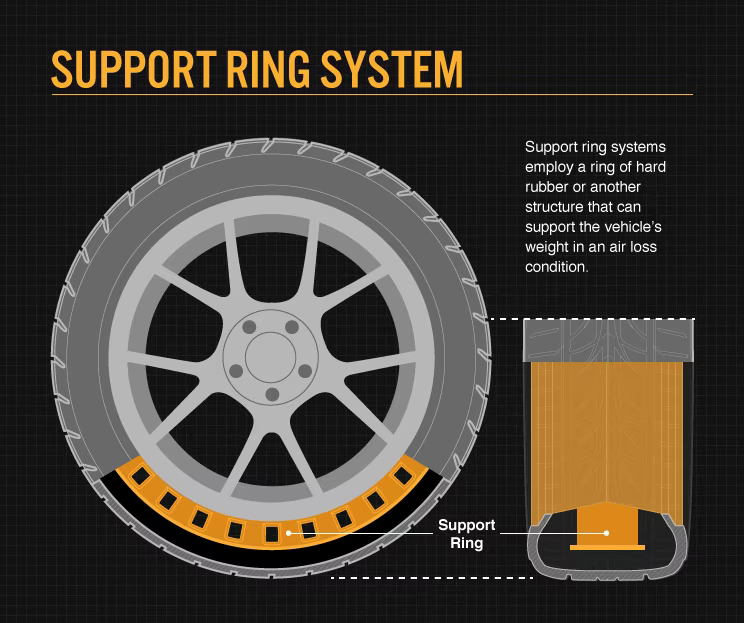
\includegraphics[width=0.5\textwidth]{images/runflat.jpg}
\end{center}

Run-flat tires have limitations, but the car is functional at reduced capacity.

\end{frame}

\begin{frame}
\frametitle{Goals}

Two distinct goals:

1. Resiliency -- carry on in the event of a failure.

2. Fail-soft -- preserve as much capability as possible or terminate gracefully.

Where did RAID fall in this spectrum?

\end{frame}

\begin{frame}
\frametitle{Resiliency}

\begin{center}
	
\includegraphics[width=0.5\textwidth]{images/rocky.jpg}
\end{center}

\end{frame}

\begin{frame}
\frametitle{Resiliency Requirements}

First question is how much resiliency you really need?


Is this ``we lose money'' or ``people might die''?



\end{frame}

\begin{frame}
\frametitle{August 29, 1997...}

\begin{center}
	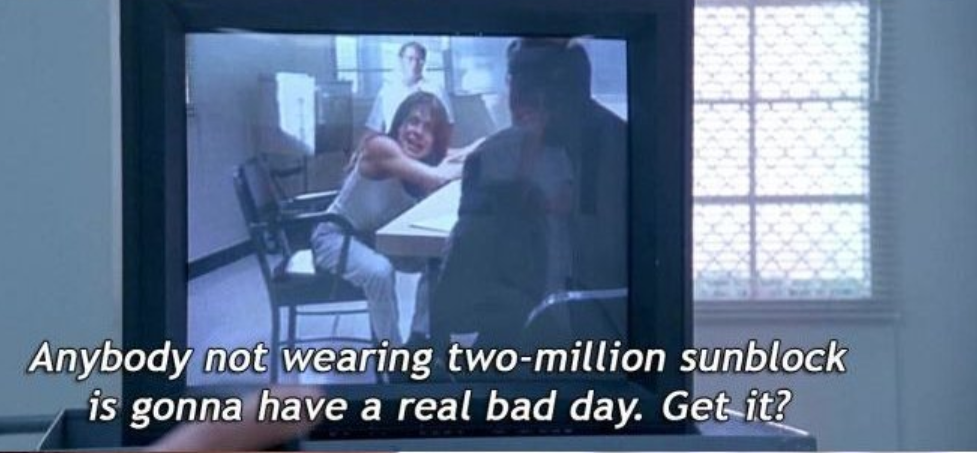
\includegraphics[width= \textwidth]{images/judgementday.png}
\end{center}

But no need to plan for nuclear armageddon (usually).

\end{frame}

\begin{frame}
\frametitle{Tradeoffs}

This is an engineering design tradeoff: how much extra capacity should we have?

\begin{center}
	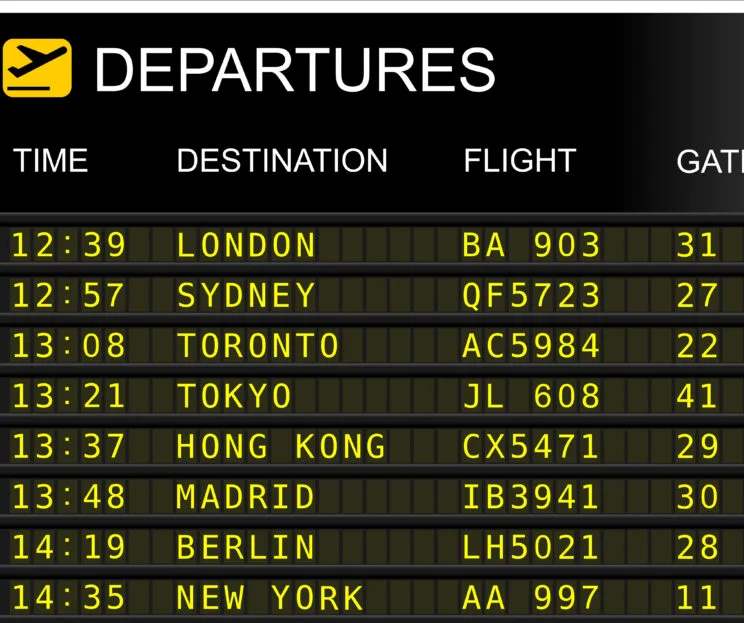
\includegraphics[width=0.5\textwidth]{images/flightdelay.jpg}
\end{center}

Too little capacity: every problem becomes global...\\
\quad Too much and we wasted money!

\end{frame}

\begin{frame}
\frametitle{Can We Fix It? Yes We Can!}

Best option for resiliency is to fix it!

Maybe not possible if this is an unrecoverable hardware failure.

Maybe deadlock detection and recovery?

\end{frame}

\begin{frame}
\frametitle{Stiff Upper Lip}

Continue as best we can at reduced capacity.

\begin{center}
	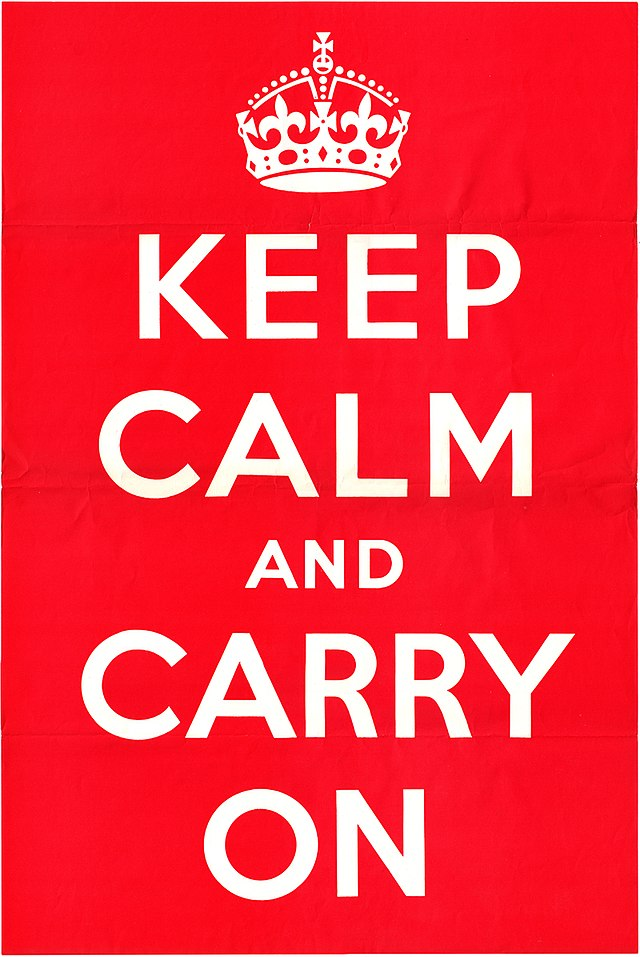
\includegraphics[width=0.4\textwidth]{images/keepcalm.jpg}
\end{center}

\end{frame}

\begin{frame}
\frametitle{Stiff Upper Lip}

Example: 4 CPU cores, all running at 50\% capacity, but one dies?

Maybe running at reduced capacity until a repair comes...

What if we can't meet all deadlines?

\end{frame}

\begin{frame}
\frametitle{Real-Time Resiliency}

The system is considered \alert{stable} if it will always meet the deadlines of its most critical tasks.

Even if lower priority tasks may not be completed at all!

Painful choices may need to be made.

\end{frame}

\begin{frame}
\frametitle{Shut It Down!}

Perhaps it's sensible to do an orderly shutdown.

Prevent data corruption, but cannot carry on.

\end{frame}

\begin{frame}
\frametitle{Stop. Hammertime.}

Cease all operation or execution immediately.

This may cause some damage, but may be the least bad choice.

\end{frame}

\begin{frame}
\frametitle{Faults and Fault Tolerance}

Until now, vague words about ``something going wrong''.

What is a fault and failure?

\end{frame}

\begin{frame}
\frametitle{Faults and Fault Tolerance}

\alert{Failure}: When the response (outcome) deviates from the specification as a result of an error.

\alert{Error}: A manifestation of a fault.

\alert{Fault}: An erroneous hardware or software state of some variety.

\end{frame}

\begin{frame}
\frametitle{Types of Fault}

\textbf{Permanent}: dead hard drive, software bug.

\textbf{Intermittent}: fault hardware chip.

\textbf{Transient}: cosmic radiation?

\end{frame}

\begin{frame}
\frametitle{Prevent Fault}

Instead of jumping right to fault tolerance, what about prevention?

\begin{center}
	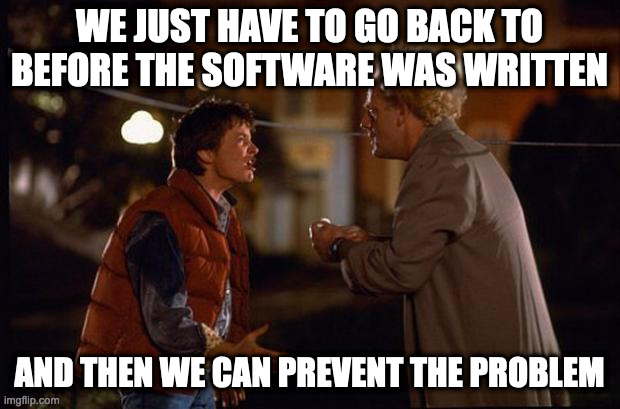
\includegraphics[width=0.5\textwidth]{images/bttf2.jpg}
\end{center}

What strategies would you use?

\end{frame}

\begin{frame}
\frametitle{Not Perfect}

Following appropriate design, implementation, and testing processes will only make faults less likely.

It is also important to resist the pressure to drop or degrade these processes when user time pressure.

Still need to think about tolerance...

\end{frame}

\begin{frame}
\frametitle{Fault Tolerance}

We already know a few things about fault tolerance from earlier topics.

\begin{center}
	
\includegraphics[width=0.5\textwidth]{images/biff.jpg}
\end{center}

Can you think of some?

\end{frame}

\begin{frame}
\frametitle{Fault Tolerance Techniques}

\begin{itemize}
	\item Process Isolation
	\item Dual-Mode Operation
	\item Preemptive, Priority-Based Scheduling
	\item Checkpoints, Transactions, Rollback
	\item RAID
	\item Checksums, Parity Bits, ECC...
\end{itemize}

\end{frame}

\begin{frame}
\frametitle{Types of Redundancy}

\alert{Information redundancy}: checksums, parity bits, ECC...

\alert{Physical redundancy}: two CPUs instead of one...

\alert{Temporal redundancy}: TCP communication, resend...

\end{frame}

\begin{frame}
\frametitle{Space Shuttle}

The Space Shuttle had both physical and temporal redundancy.

\begin{center}
	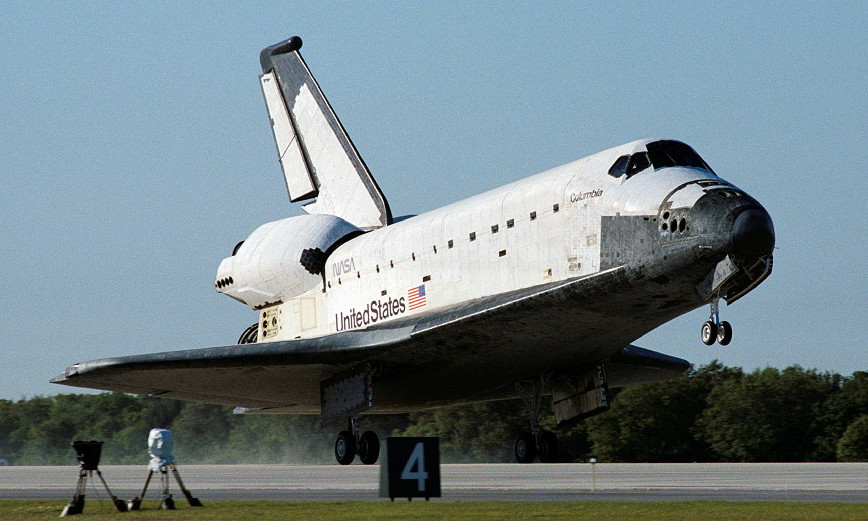
\includegraphics[width=0.5\textwidth]{images/spaceshuttle.jpg}
\end{center}

Important thing: no single point of failure!

\end{frame}

\begin{frame}
\frametitle{Now I Have Two Problems}


\begin{center}
	
\includegraphics[width=0.4\textwidth]{images/achievement.jpg}
\end{center}

We covered this a little bit in the Byzantine Generals Problem.

We'll consider one in particular: clock synchronization.

\end{frame}

\begin{frame}
\frametitle{Clock Synchronization}

It is not trivial to get two independent systems to agree on what time it is.

\begin{center}
	
\includegraphics[width=0.4\textwidth]{images/jumanji.jpg}
\end{center}

Inevitably, all clocks except the universal reference clock are off by some amount; it's just a question of how much! 

\end{frame}

\begin{frame}
\frametitle{Disagreement Means Problems}

It's easy to imagine scenarios where independent systems who don't agree on what time it is will misbehave.

Ever been in a video call with lag?

Time zones also matter!

\end{frame}

\begin{frame}
\frametitle{Quartz Clocks}

Clocks frequently use quartz for synchronization, but there is always drift and measurement error.

A quartz clock will typically vary by about half a second per day, so the idea of systems being off by a full second is quite reasonable.


Just imagine System A is fast by 0.5s and System B is slow by 0.5s.

\end{frame}

\begin{frame}
\frametitle{Time Travel is Real}

In a non-real time operating system, it's often okay to just change the clock to the correct time and just jump there.

But for a real-time system, breaking the expectation of linear time can cause events to run again, so typically we do not wish to do that.

The solutions are effectively a graduated slowdown or speedup... but to when?

\end{frame}

\begin{frame}
\frametitle{NTP}
A possible solution is something like the Network Time Protocol.

Effectively, it's difficult or impossible to get more than one system to agree on what time it is. 

Better: build your system to account for these things.

\end{frame}

\begin{frame}
\frametitle{Distributed Systems Course}

All of this is just a very simple overview of some of the issues that might arise when we have multiple systems for redundancy. 

This is a complicated subject and is a whole 4th year ECE technical elective that you could take!


\end{frame}

\end{document}

